\subsection{Ερώτημα 3-2}

Σε αυτό το τμήμα της άσκησης εξετάζουμε την επίδοση των κάτωθι διαφορετικών
τοπολογιών που διαφέρουν μεταξύ τους ως προς τον διαμοιρασμό των κρυφών μνημών.
Συγκεκριμένα εξετάζουμε τις ακόλουθες τοπολογίες:

\begin{itemize}
   \item share-all: και τα 4 νήματα βρίσκονται σε πυρήνες με κοινή L2 cache
   \item share-L3: και τα 4 νήματα βρίσκονται σε πυρήνες με κοινή L3 cache, αλλά όχι κοινή L2
   \item share-nothing: και τα 4 νήματα βρίσκονται σε πυρήνες με διαφορετική L3 cache 
\end{itemize}

\begin{minipage}{\textwidth}
   \begin{center}
      \vspace{10mm}
      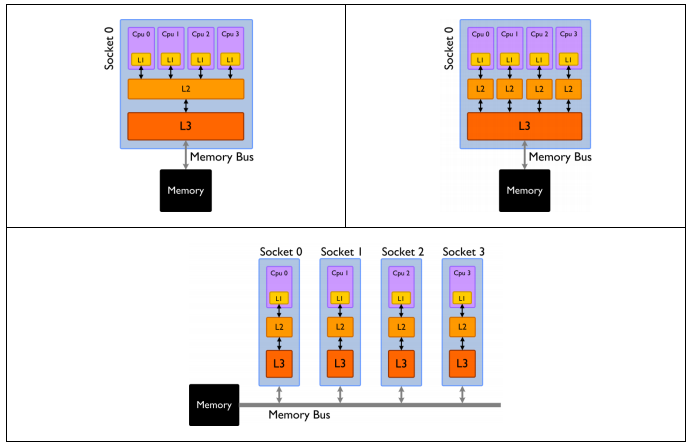
\includegraphics[width=0.9\textwidth]{./imgs/topologies.png}
      \vspace{6mm}
   \end{center}
\end{minipage}

\noindent Στη συνέχεια ακολουθούν ραβδογράμματα τα οποία παρουσιάζουν τους χρόνους
εκτέλεσης, την κατανάλωση ενέργειας και την μετρική EDP για τα configurations
αυτά:

\begin{minipage}{\textwidth}
   \begin{center}
      \fbox{\textlatin{\textbf{\textit{Time analysis}}}}\\
      \vspace{3mm}
      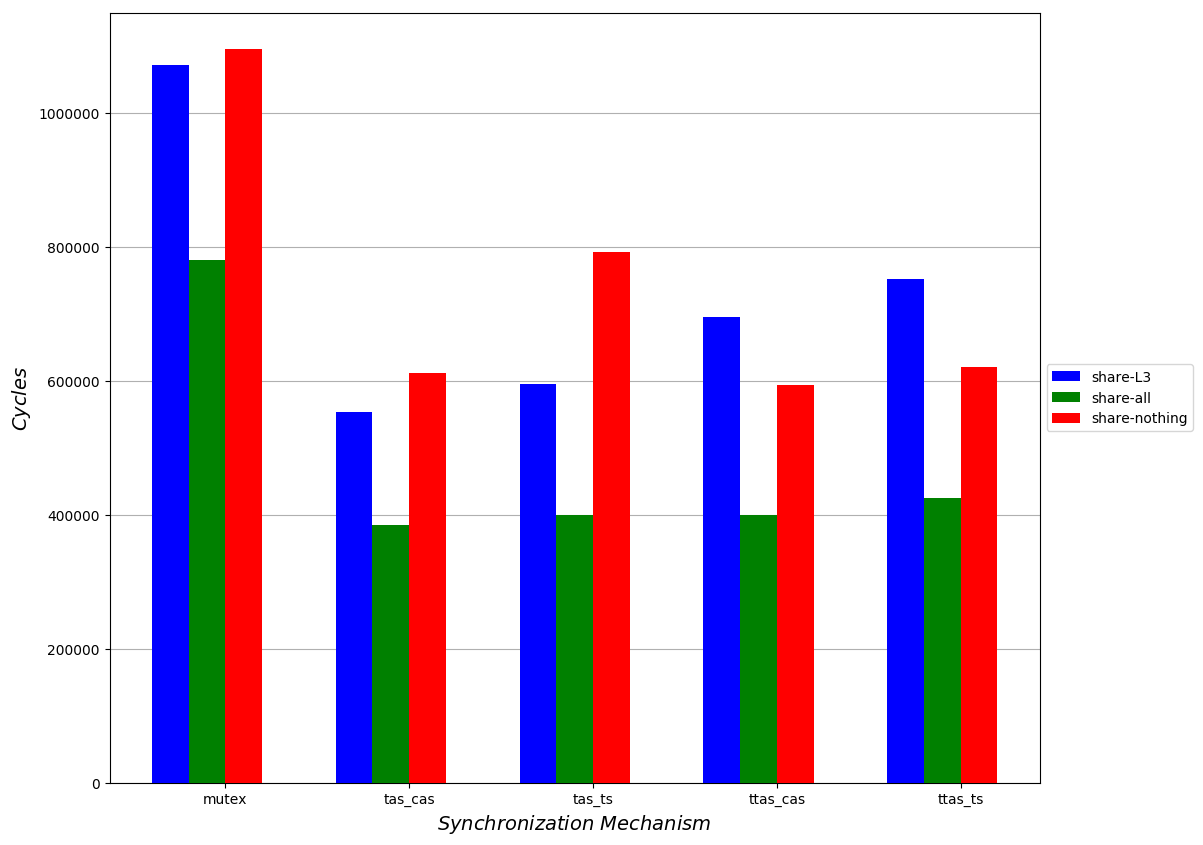
\includegraphics[width=0.75\textwidth, frame]{./graphs/sniper/threads/topology-time-analysis.png}
      \vspace{6mm}
   \end{center}
\end{minipage}

\begin{minipage}{\textwidth}
   \begin{center}
      \fbox{\textlatin{\textbf{\textit{Energy Analysis}}}}\\
      \vspace{3mm}
      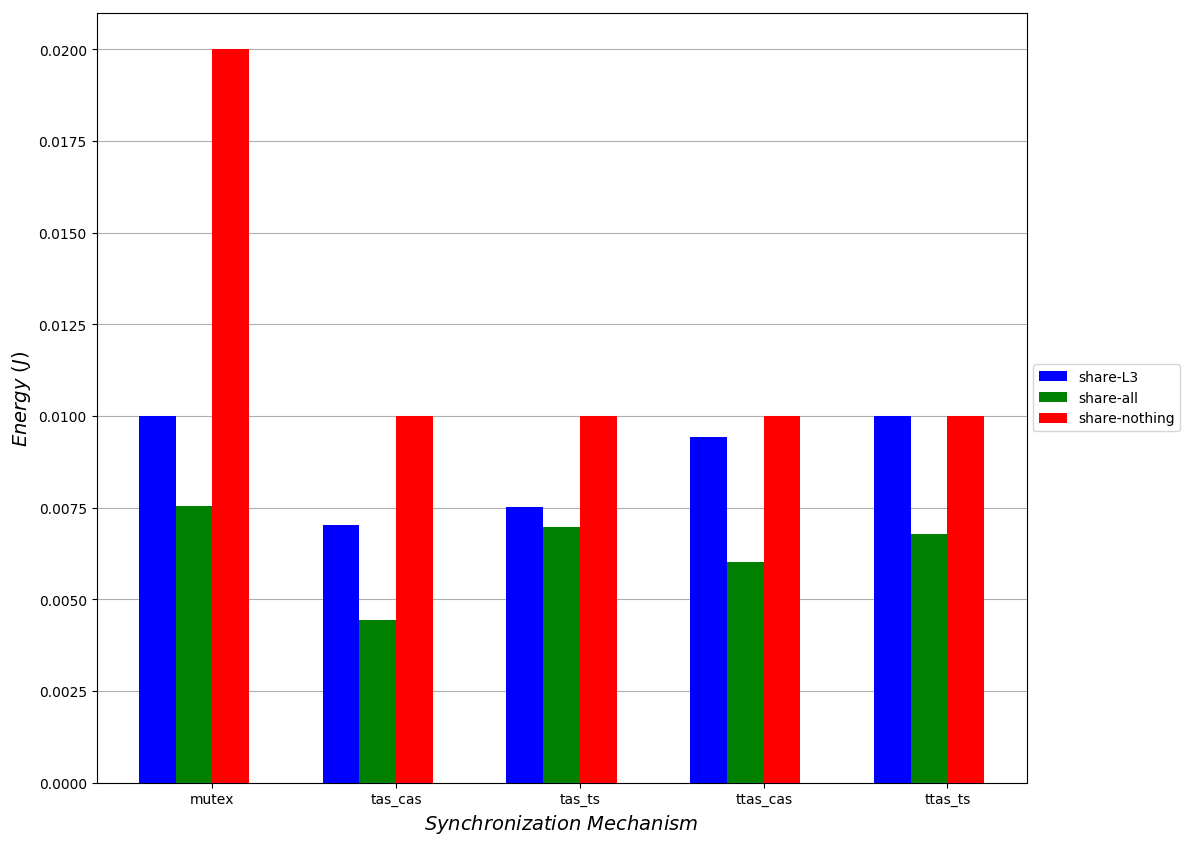
\includegraphics[width=0.75\textwidth, frame]{./graphs/sniper/threads/topology-energy-analysis.png}
      \vspace{6mm}
   \end{center}
\end{minipage}

\begin{minipage}{\textwidth}
   \begin{center}
      \fbox{\textlatin{\textbf{\textit{EDP Analysis}}}}\\
      \vspace{3mm}
      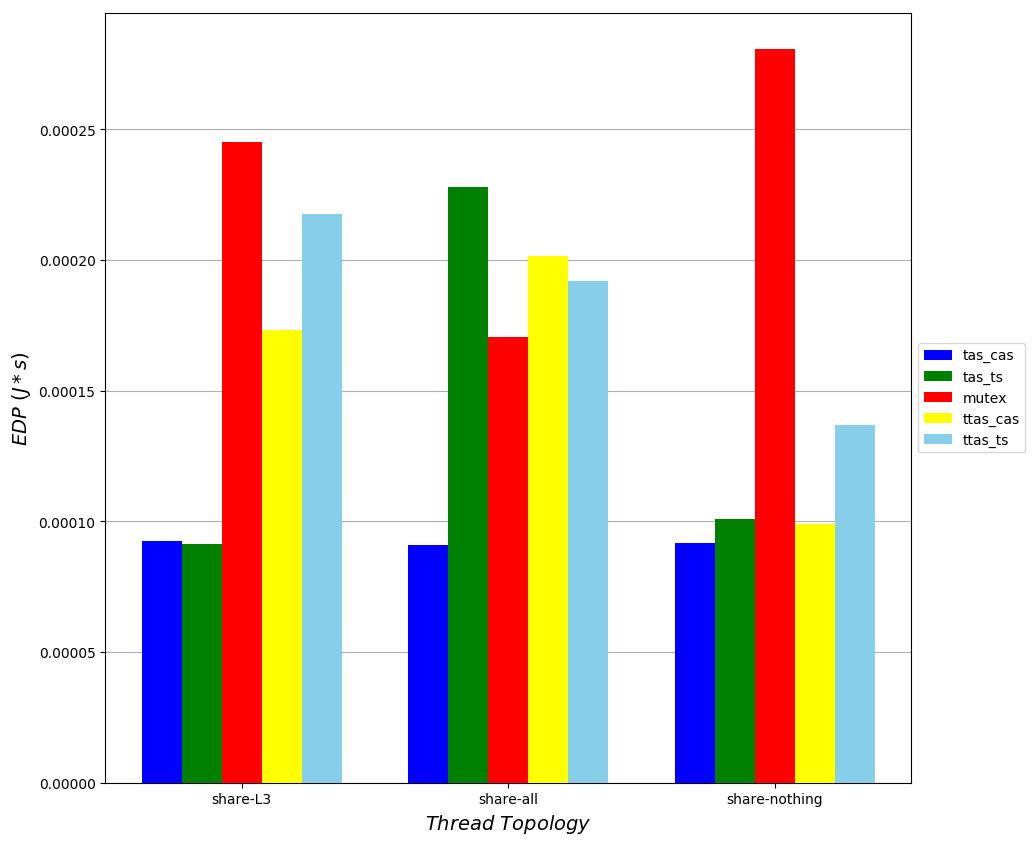
\includegraphics[width=0.75\textwidth, frame]{./graphs/sniper/threads/topology-edp-analysis.png}
      \vspace{6mm}
   \end{center}
\end{minipage}

\paragraph{Συμπεράσματα - Σχόλια}
Όσον αφορά την επίδοση με βάση τη μετρική του χρόνου (ή αντίστοιχα κύκλος
εκτέλεσης) για όλους τους υπο μελέτη μηχανισμούς συγχρονισμου, την καλύτερη
επίδοση λαμβάνουμε στην τοπολογία \textbf{share-all}. Για τους μηχανισμούς
συγχρονισμού MUTEX, TAS\_TS, TAS\_CAS οι τοπολογίες σε φθίνουσα επίδοση είναι οι
share-all, share-L3, share-nothing. Για τους μηχανισμούς συγχρονισμού TTAS\_TS,
TTAS\_CAS οι τοπολογίες σε φθίνουσα επίδοση είναι οι share-all, share-nothing,
share-L3. Η βέλτιστη επίδοση του share-all αιτιολογείται από το γεγονός οτι αν
επεξεργαστής ζητήσει ένα Invalid cache line θα ενημερωθεί η ιεραρχία μνήμης
μέχρι την L2 και θα το διαβάσει από εκεί, ενώ στο share-L3 η invalid cache line
θα ζητηθεί από την L3 και για share-nothing φτάνουμε μέχρι και την κύρια μνήμη
για κάθε αυξάνοντας σημαντικά τον χρόνο που απαιτείται, αφού όσο πιο "μακριά"
ιεραρχικά βρίσκεται μία μνήμη από τον επεξεργαστή τόσο πιο αργή είναι.

Ως προς την κατανάλωση ενέργειας την μεγαλύτερη κατανάλωση έχουμε στην τοπολογία 
share-nothing, ενώ την μικρότερη κατανάλωση στην τοπολογία share-all. Αντίστοιχα,
με κριτήριο την EDP μετρική, την καλύτερη επίδοση έχει η τπολογία share-all.
\vspace{1em}

\noindent Ακολουθεί η υλοποίηση των μηχανισμών στο αρχείο lock.h: \vspace{0.5cm}
\lstinputlisting[language=C++, numbers=left, frame = single, basicstyle=\small]{lock.h}
